%%%%%%%%%%%%%%%%%%%%%%%%%%%%%%%%%%%%%%%%%%%%%%%%%%%%
% 10-minute version — non-expert audience
% Structure: Challenges → Scientific solution → Pipeline & platform
%%%%%%%%%%%%%%%%%%%%%%%%%%%%%%%%%%%%%%%%%%%%%%%%%%%%

\documentclass{beamer}

% Theme + packages
\usepackage{otherResources/presentazione_allPackages}
\usepackage{tikz}
\usetikzlibrary{positioning,calc,arrows.meta,fit,backgrounds,matrix,shapes.geometric,decorations.pathreplacing}

% Metadata
\hypersetup{
	pdfauthor={Nicola Perin},
	pdftitle={Designing and deploying a FAIR-by-design data pipeline and platform for electron microscopy laboratories},
	pdfsubject={Research thesis in: Data Management}
}

\title[FAIR-by-design EM pipeline]{Designing and deploying a FAIR-by-design data pipeline and platform for electron microscopy laboratories}
\subtitle{Research thesis in Data Management}
\institute{University of Trieste}
\author[Nicola Perin]{Nicola Perin}
\year=2025
\month=09
\day=19
\date{\the\day/\the\month/\the\year}
% Advisor labels
\def\relatore{Dr. Federica Bazzocchi}
\def\relatoreLabel{Supervisor}
\def\candidatoLabel{Candidate}

% Logos
\def\LogoUniversita{otherResources/Units.Logo3Righe.png}
\def\LogoDipartimento{otherResources/DSSC_logo.png}
\def\LogoFiligrana{otherResources/background-blu.png}

% Apply your theme
%%%%%%%%%%%%%%%%%%%%%%%%%%%%%%%%%%%%%%%%%%%%%%%%%%%%%%%%%%%
%
% Copyright 2022 by Isac Pasianotto
%
% This file may be distributed and/or modified
%
% 1. under the LaTeX Project Public License and/or
% 2. under the GNU Public License.
%
%%%%%%%%%%%%%%%%%%%%%%%%%%%%%%%%%%%%%%%%%%%%%%%%%%%%%%%%%%%

%% 	Variabili di tipo "color": 

\definecolor{bluUnits100}{rgb}{0.16,0.22,0.36} 
\definecolor{bluUnits80}{rgb}{0.22,0.3,0.51}
\definecolor{bluUnits70}{rgb}{0.25,0.35,0.58}
\definecolor{bluUnits50}{rgb}{0.41,0.51,0.74}
\definecolor{bluUnits40}{rgb}{0.56,0.63,0.81}
\definecolor{bluUnits25}{rgb}{0.78,0.82,0.9}
\definecolor{bluUnits10}{rgb}{0.93,0.94,0.96}
\definecolor{grey}{rgb}{0.3686, 0.5255, 0.6235} 

%%	Palette di colori 

\setbeamercolor{palette primary}{bg=bluUnits100,fg=white}
\setbeamercolor{palette secondary}{bg=bluUnits80,fg=bluUnits25}
\setbeamercolor{palette tertiary}{bg=bluUnits50,fg=bluUnits100}
\setbeamercolor{palette quaternary}{bg=bluUnits40,fg=white}
\setbeamercolor{palette light primary}{bg=bluUnits25,fg=bluUnits100}
\setbeamercolor{palette titleframe}{bg=bluUnits10, fg=bluUnits80}


		%%%%%%%%%%%%%%%%%%%%%%%%%%%%%%%%%%
		%% Impostazioni generali slide  %%
		%%%%%%%%%%%%%%%%%%%%%%%%%%%%%%%%%%

%%	Setta l'immagine da mettere come sfondo, riducendone l'opacità
\usebackgroundtemplate{\tikz\node[opacity=0.1]{\includegraphics[height=\textheight]{\LogoFiligrana}};}

%%	Elenchi puntati, numerati, etc.

\setbeamercolor{structure}{fg=bluUnits80}
\setbeamertemplate{enumerate item}[circle]
\setbeamertemplate{itemize subitem}[ball]
% Valutare a secoda del contesto se sostituire con 
% \setbeamertemplate{items}[circle]
\setbeamercolor{alerted text}{fg=bluUnits50}

%% 	Colore delle scritte nella presentazione

\setbeamercolor{normal text}{fg=bluUnits100,bg=white}

%% 	Settaggio della linea in alto (headline)

\setbeamertemplate{headline}{
	\vskip1pt
	\leavevmode	
	\hbox{
		\begin{beamercolorbox}[wd=.99\paperwidth,ht=2.5ex,dp=1.125ex]{palette light primary}
			\insertsectionnavigationhorizontal{\paperwidth}{}{\hskip0pt plus1filll}
		\end{beamercolorbox}
	}
}

%%	Settaggio riga in basso (footline) 
 
\setbeamertemplate{footline}{
       \leavevmode
	   \hbox{
           \begin{beamercolorbox}[wd=.2\textwidth,ht=2.6ex,dp=1ex,center]{palette tertiary}
		    \usebeamerfont{author in head/foot}\insertshortauthor
    	\end{beamercolorbox}
	
    	\begin{beamercolorbox}[wd=.27\textwidth,ht=2.6ex,dp=1ex,center]{palette quaternary}
	   		\usebeamerfont{institute in head/foot}\insertshortinstitute
	   	\end{beamercolorbox}
	
    	\begin{beamercolorbox}[wd=.40\textwidth,ht=2.6ex,dp=1ex,center]{palette primary}
    		\usebeamerfont{title in head/foot}\insertshorttitle
    	\end{beamercolorbox}

    	\begin{beamercolorbox}[wd=.1\textwidth,ht=2.6ex,dp=1ex,center]{palette light primary}
	   		\insertframenumber{}/\inserttotalframenumber
	    \end{beamercolorbox}
    }
    \vskip2pt

}

%%	Settaggio tittoli delle slide  

\setbeamertemplate{frametitle}{
	\begin{beamercolorbox}[wd=\paperwidth,ht=2.75ex,dp=1ex,left]{palette titleframe}
		\qquad \textbf{\insertframetitle}
	\end{beamercolorbox}
}


		%%%%%%%%%%%%%%%%%%%%%%%%%%%%%%%
		%% Impostazioni Prima Slide  %%
		%%%%%%%%%%%%%%%%%%%%%%%%%%%%%%%
	
	
	
	
		
\def\setTitlestyleDissertation{
	
	\defbeamertemplate*{title page}{customized}[1][]{
		
		%  Commentare il seguente ambiente {center} e decommentare {flushright} quello successivo in caso
		%	si voglia usare solo il logo dell'UNI
		
		\begin{center}
			\begin{multicols}{2}
				\includegraphics[width=0.45\textwidth]{\LogoDipartimento}
			\columnbreak
				\includegraphics[width=0.45\textwidth]{\LogoUniversita}		
			\end{multicols}
		\end{center}
	
		%	\begin{flushright}
		%		\includegraphics[width=0.45\textwidth]{\LogoUniversita}	
		%	\end{flushright}
	
		\smallskip
		
		\begin{center}		
			\usebeamerfont{title}\textbf{\inserttitle}\par
			\usebeamerfont{subtitle}\usebeamercolor[fg]{subtitle}\insertsubtitle\par
			\medskip		
			
			%% Il seguente layout dentro l'ambiente multicols serve per le tesi.
			
			\begin{multicols}{2}
				\begin{tabular}{c}
					\usebeamerfont{normal text}{\relatoreLabel} \\
					\usebeamerfont{author}{\relatore}
					
						% Decommentare in caso siano presenti dei correlatori
					%\\
					%\usebeamerfont{normal text}{\correlatoreLabel} \\
					%\usebeamerfont{author}{\correlatore}
						
				\end{tabular}					
				\columnbreak
				\begin{tabular}{c}
					\candidatoLabel \\
					\usebeamerfont{author}{\insertauthor}
				\end{tabular}
			\end{multicols}
		
			\par
			
			\bigskip  	% --> nel caso di relatore e basta
			%\smallskip 	% --> nel caso di relatore + correlatore
			
			\insertinstitute\par
			
			\bigskip	% --> nel caso di relatore e basta
			%\smallskip	% --> nel caso di relatore + correlatore
			
			\usebeamerfont{date}\insertdate\par
			
			\bigskip	% --> nel caso di relatore e basta
			%\smallskip	% --> nel caso di relatore + correlatore
		\end{center}
	}
}


\begin{document}

	% =====================
	% 0) Title
	% =====================
	\begin{frame}
		\setTitlestyleDissertation
		\maketitle
	\end{frame}
	
	% =====================
	% 1) Orientation
	% =====================
	\begin{frame}
		\frametitle{Outline}
		\large
		\begin{enumerate}
			\item Data management challenges in electron microscopy
			\item Scientific foundations: FAIR data and standards
			\item Our infrastructure: LAME and ORFEO
			\item Pipeline and platform design
		\end{enumerate}
	\end{frame}
	
	% =====================
	% 2) Challenges
	% =====================
\begin{frame}
	\frametitle{Electron microscopy and its data challenges}
	\begin{columns}[T,totalwidth=\textwidth]
		% --- Left column: text ---
		\column{0.6\textwidth}
		\begin{itemize}
			\item \textbf{Electron microscopy (EM)}: probe matter at the nanometer scale.
			\item Techniques: TEM (internal), SEM (surface), STEM (combo + spectroscopy).
			\item Produces huge datasets: images, diffraction patterns, spectra.
			\item Issues:
			\begin{itemize}
				\item Terabytes per session, proprietary formats, poor metadata.
				\item Manual handling → lost context.
				\item Hard to share and reuse.
			\end{itemize}
		\end{itemize}
		
		% --- Right column: image ---
		\column{0.40\textwidth}
		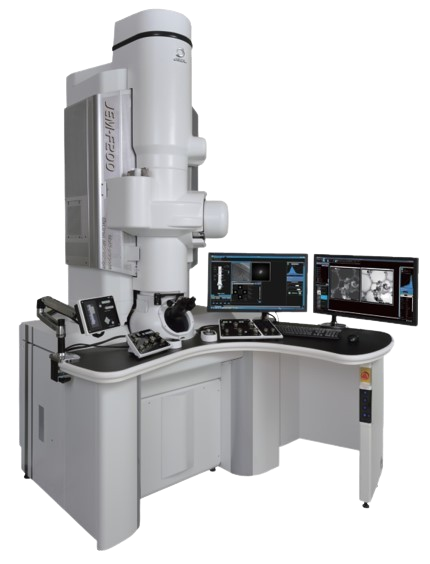
\includegraphics[width=\linewidth]{otherResources/LAME_microscope.png}
	\end{columns}
	
	\vspace{0.4em}
	\small\itshape Question: how to keep EM data usable and shareable in the long run?
\end{frame}

	
	
	% =====================
	% Scientific solution – FAIR + NeXus/NXem
	% =====================
	\begin{frame}
		\frametitle{Scientific solution: FAIR and standards}
		\begin{columns}[T,totalwidth=\textwidth]
			\column{0.60\textwidth}
			\begin{itemize}
				\item \textbf{FAIR} = Findable, Accessible, Interoperable, Reusable.  
				Goal: data remain useful beyond the lab and the project.
				\item \textbf{NeXus}: international standard on top of HDF5 for structured scientific data  
				(e.g. \texttt{NXinstrument}, \texttt{NXsample}).
				\item \textbf{NXem}: new NeXus application definition for electron microscopy.  
				Ensures images, diffraction, spectra and metadata are stored consistently.
			\end{itemize}
			\column{0.4\textwidth}
			
\includegraphics[width=\linewidth]{otherResources/FAIR_data_principles.png}\\[0.5em]
			
\includegraphics[width=\linewidth]{otherResources/NEXUS_logo.png}
		\end{columns}
	\end{frame}
	
	% =====================
	% 5) Scientific solution – NFFA-DI
	% =====================
	\begin{frame}
		\frametitle{Scientific solution: NFFA-DI}
		\begin{columns}[T,totalwidth=\textwidth]
			\column{0.55\textwidth}
			\begin{itemize}
				\item \textbf{NFFA-DI} = Nano Foundries and Fine Analysis – Digital Infrastructure.
				\item National initiative linking nanoscience labs across Italy.
				\item Mission: \textbf{FAIR data practices}, open access to advanced instruments, shared compute.
				\item My work contributes to this broader infrastructure effort.
			\end{itemize}
			\column{0.52\textwidth}
			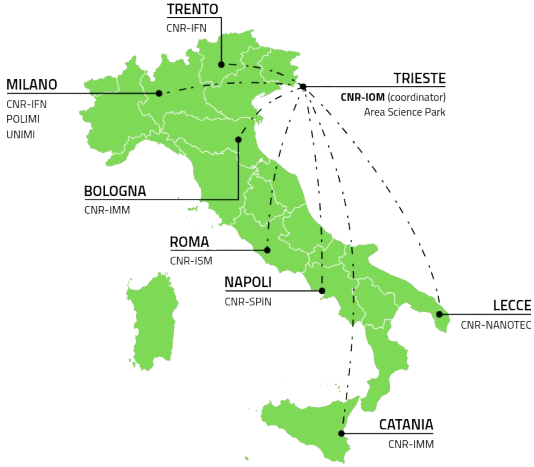
\includegraphics[width=\linewidth]{otherResources/NFFA_map.png}
			\vspace{1em}
			\tiny Source: \url{https://nffa-di.it/en/}
		\end{columns}
	\end{frame}
	
	\begin{frame}
		\frametitle{Our infrastructure: LAME and ORFEO}
		\begin{itemize}
			\item \textbf{LAME}: advanced EM lab (opened 2022), with TEM/STEM and SEM; affiliated with NFFA-DI.
			\item \textbf{ORFEO}: datacenter providing storage, HPC, identity services.  
			Core of the NFFA-DI digital infrastructure.
			\item \textbf{Current gap:} local storage, manual transfers, no smooth link to ORFEO.
		\end{itemize}
		\vspace{1em}
		\centering
		\begin{tikzpicture}[>=Stealth,thick]
			% LAME microscope
			\node (lame) at (0,0) {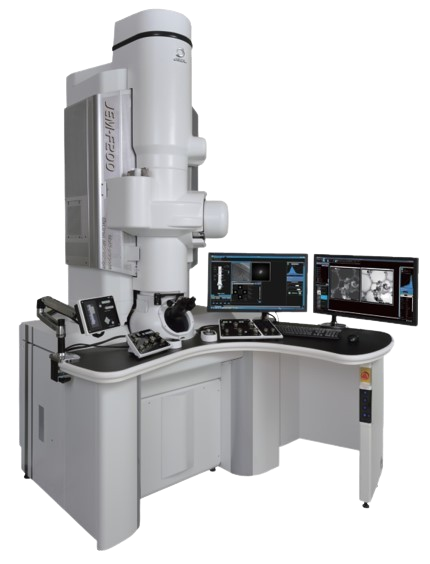
\includegraphics[width=0.28\linewidth]{otherResources/LAME_microscope.png}};
			% ORFEO datacenter (shifted further to the right)
			\node (orfeo) at (6,0) {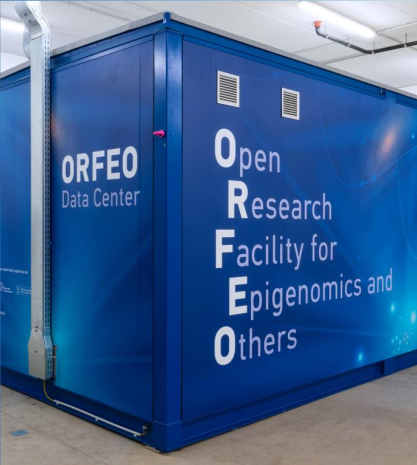
\includegraphics[width=0.28\linewidth]{otherResources/ORFEO.png}};
			% Arrow
			\draw[->, line width=1mm, blue!70!black] (lame.east) -- (orfeo.west);
		\end{tikzpicture}
	\end{frame}
	
	% =====================
	% Pipeline as solution
	% =====================
	\begin{frame}
		\frametitle{Practical solution: a FAIR-by-design pipeline}
		\begin{itemize}
			\item Bridges \textbf{LAME lab practices} with \textbf{ORFEO infrastructure}.
			\item Ensures data move \textbf{smoothly from capture to reuse}, without manual gaps.
			\item FAIRification happens at the \textbf{standardization step}.
			\item A \textbf{web application} orchestrates transfer, standardization, and storage.
		\end{itemize}
		\vspace{1em}
		\centering
		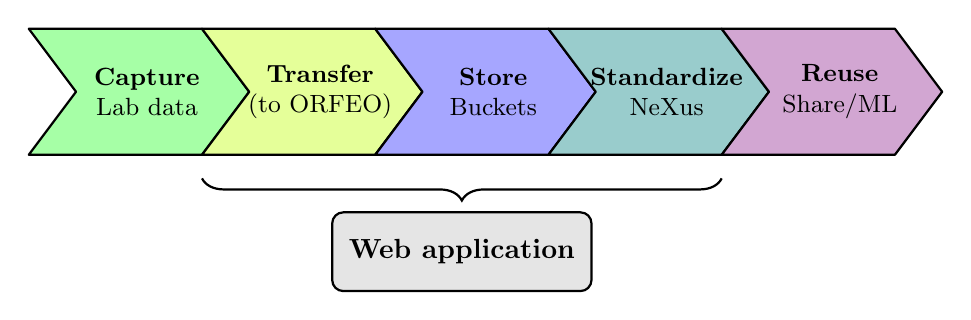
\begin{tikzpicture}[thick,>=Stealth]
			% geometry (smaller chevrons)
			\def\H{1.6} \def\W{2.2} \def\TIP{0.6}
			\pgfmathsetmacro{\HalfH}{0.5*\H}
			\pgfmathsetmacro{\MidX}{0.5*\W}
			\pgfmathsetmacro{\WplusTIP}{\W+\TIP}
			
			% Capture
			\begin{scope}[shift={(-0.2,0)}]
				\path[draw=black, fill=green!35, line join=round]
				(0,0) -- (\W,0) -- (\WplusTIP,\HalfH) -- (\W,\H) -- (0,\H) -- (\TIP,\HalfH) -- cycle;
				\node[align=center, font=\small, xshift=4mm] at (\MidX,\HalfH) {\textbf{Capture}\\Lab data};
			\end{scope}
			
			% Transfer
			\begin{scope}[shift={(2.0,0)}]
				\path[draw=black, fill=lime!40, line join=round]
				(0,0) -- (\W,0) -- (\WplusTIP,\HalfH) -- (\W,\H) -- (0,\H) -- (\TIP,\HalfH) -- cycle;
				\node[align=center, font=\small, xshift=4mm] at (\MidX,\HalfH) {\textbf{Transfer}\\(to ORFEO)};
			\end{scope}
			
			% Store
			\begin{scope}[shift={(4.2,0)}]
				\path[draw=black, fill=blue!35, line join=round]
				(0,0) -- (\W,0) -- (\WplusTIP,\HalfH) -- (\W,\H) -- (0,\H) -- (\TIP,\HalfH) -- cycle;
				\node[align=center, font=\small, xshift=4mm] at (\MidX,\HalfH) {\textbf{Store}\\Buckets};
			\end{scope}
			
			% Standardize
			\begin{scope}[shift={(6.4,0)}]
				\path[draw=black, fill=teal!40, line join=round]
				(0,0) -- (\W,0) -- (\WplusTIP,\HalfH) -- (\W,\H) -- (0,\H) -- (\TIP,\HalfH) -- cycle;
				\node[align=center, font=\small, xshift=4mm] at (\MidX,\HalfH) {\textbf{Standardize}\\NeXus};
			\end{scope}
			
			% Reuse
			\begin{scope}[shift={(8.6,0)}]
				\path[draw=black, fill=violet!35, line join=round]
				(0,0) -- (\W,0) -- (\WplusTIP,\HalfH) -- (\W,\H) -- (0,\H) -- (\TIP,\HalfH) -- cycle;
				\node[align=center, font=\small, xshift=4mm] at (\MidX,\HalfH) {\textbf{Reuse}\\Share/ML};
			\end{scope}
			
			% Curly brace below Transfer+Store+Standardize
			\draw [decorate,decoration={brace,amplitude=8pt,mirror},thick]
			(2.0,-0.3) -- (8.6,-0.3) node[midway, yshift=-0.6cm] (brace) {};
			
			% Webapp box
			\node[
			draw,
			fill=gray!20,
			rounded corners,
			minimum height=1cm,
			inner sep=6pt,
			yshift=-0.2cm        % shift upwards (closer to brace)
			] at (brace.south) {\textbf{Web application}};
			
		\end{tikzpicture}
	\end{frame}
	
	% =====================
	% Webapp and infrastructure
	% =====================
	\begin{frame}
		\frametitle{Designing the web application}
		
		\textbf{The infrastructure}
		\begin{itemize}
			\item \textbf{Authentik}: centralized single sign-on (SSO).
			\item \textbf{Ceph storage}: a distributed object store.  
			Data are split into \textbf{objects}, replicated across many servers → scalable and fault-tolerant.
		\end{itemize}
		
		\vspace{0.8em}
		
		\textbf{The application}
		\begin{itemize}
			\item Built with \textbf{Django}, modeling research workflow as:  
			
			\textbf{Project / Proposal / Sample / Experiment / Measure}.
			\item Manages user identities through Authentik.
			\item Interacts with Ceph via the \textbf{Amazon S3 API}.
			\item Runs \textbf{background tasks} (NeXus conversion).
		\end{itemize}
	\end{frame}
	
	% =====================
	% Using the web application in practice
	% =====================
	\begin{frame}[t]
		\frametitle{Using the web application}
		
		%----- top row: text (left) + sample form (right) -----
		\begin{columns}[T,onlytextwidth]
			% Left: numbered list
			\column{0.55\textwidth}
			\begin{enumerate}
				\item Log in with credentials.
				\item Create a project, add samples and experiments.
				\item Upload raw data files.
			\end{enumerate}
			
			% Right: sample form with thin black border
			\column{0.42\textwidth}
			\centering
			\vspace{-1.6em}
			\begin{tikzpicture}
				\node[
				inner sep=0, outer sep=0, % eliminate padding
				draw=black, thin
				] {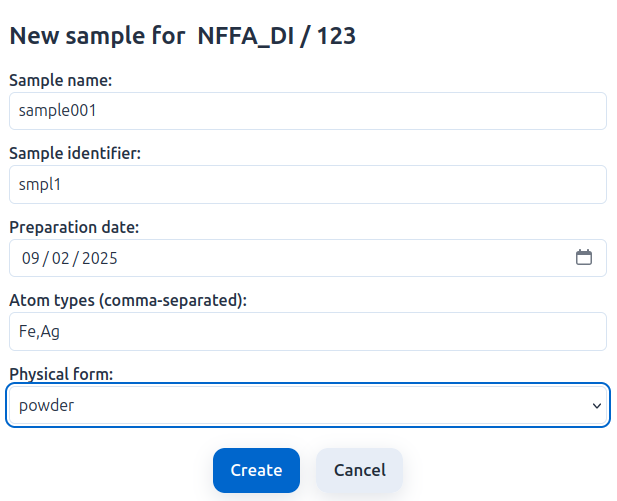
\includegraphics[width=\linewidth]{otherResources/ui_modal_new_sample_slim.png}};
			\end{tikzpicture}
		\end{columns}
		
		%----- reserve space for the bottom image -----
		\newlength{\bottomimgheight}
		\setlength{\bottomimgheight}{0.36\paperheight}
		\vspace*{\bottomimgheight}
		
		%----- bottom image spanning the frame, with border -----
		\begin{tikzpicture}[remember picture,overlay]
			\node[
			anchor=south,
			yshift=0.7cm,
			inner sep=0, outer sep=0,
			draw=black, thin
			] at (current page.south)
			{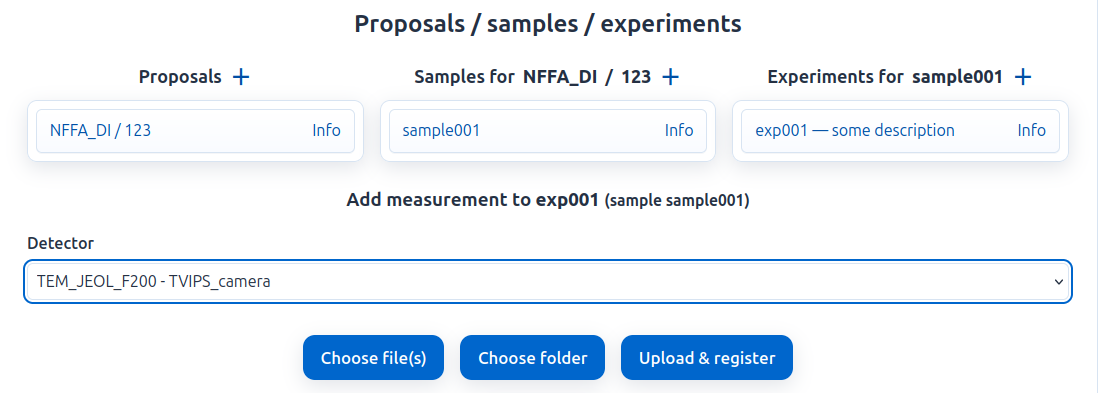
\includegraphics[width=0.85\paperwidth]{otherResources/ui_add_measurement_slim.png}};
		\end{tikzpicture}
	\end{frame}
	
	\begin{frame}
		\frametitle{Testing \& deployment: \textit{VirtualOrfeo}}
		\begin{itemize}
			\item A lightweight clone of the ORFEO datacenter.
			\item Same configuration as production (K3s cluster, storage, identity). 
			\item Allowed realistic testing of the pipeline before deployment.
			\item Reduced risk by validating uploads, NeXus conversion, and access control in a safe environment.
		\end{itemize}
	\end{frame}
	
	\begin{frame}
		\frametitle{Conclusions}
		
		\begin{itemize}
			\item \textbf{Pipeline}: from lab capture to FAIR data in ORFEO.
			\item \textbf{Webapp}: practical tool for projects, uploads, and NeXus conversion.
			\item \textbf{Validation}: tested end-to-end on VirtualOrfeo.
			\item \textbf{Impact}: reusable design for NFFA-DI and other labs.
			\item \textbf{Next}: tighter metadata automation, integration with analysis workflows.
		\end{itemize}
	\end{frame}
	
	% =====================
	% 11) Thanks
	% =====================
	\begin{frame}
		\centering
		\vfill
		{\Huge \textbf{Thank you!}}\\[1.2em]
		{\large Questions welcome.}
		\vfill
	\end{frame}
	
\end{document}
